\tikzstyle{block} =[rectangle, draw, fill=blue!20, text width = 5em, text centered, rounded corners, minimum height = 4em]
\tikzstyle{line} = [draw, ->]

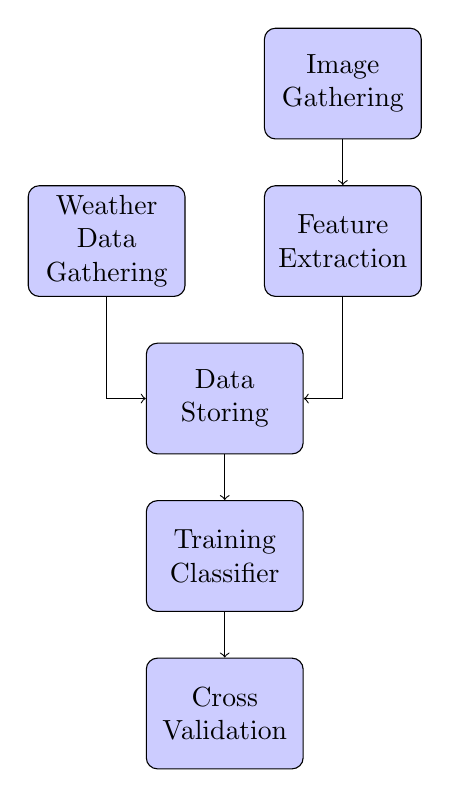
\begin{tikzpicture}[node distance = 2cm, auto]

  \node[block] (image) {Image Gathering};
  \node[block, below of = image] (feature) {Feature Extraction};
  \node[block, left of = feature, node distance = 3cm] (weather) {Weather Data Gathering};
  \node[block, below of = weather, xshift = 1.5cm] (storing) {Data Storing};
  \node[block, below of = storing] (training) {Training Classifier};
  \node[block, below of = training] (cross) {Cross Validation};

  \path [line] (image) -- (feature);
  \path [line] (feature) |- (storing);
  \path [line] (weather) |- (storing);
  \path [line] (storing) -- (training);
  \path [line] (training) -- (cross);

\end{tikzpicture}
